\documentclass[conference]{IEEEtran}

\usepackage{cite}
\usepackage{amsmath}
\usepackage{graphicx}
\usepackage{booktabs}
\usepackage{url}
\usepackage{xcolor}
\usepackage{multirow}
\usepackage{array}

\graphicspath{{images/}{../outputs/experiments/citation-analysis/}{../outputs/experiments/annotation-analysis/}}

\begin{document}

\title{Auditing AI-Generated Draft Judgments: Citation Provenance, Holding Accuracy, and Reasoning Grounding}

\author{\IEEEauthorblockN{Roopa Raj}
\IEEEauthorblockA{School of Computing\\
Ulster University\\
Belfast, UK\\
Raj-R@ulster.ac.uk}}

\maketitle

\begin{abstract}
Retrieval-augmented generation (RAG) systems are increasingly proposed for judicial decision support, yet the presence of a legal knowledge base does not guarantee that generated outputs are accurate. As regulators increasingly classify judicial AI as high-risk, structured evaluation methods are needed before deployment. This paper audits 59 AI-generated draft judgments produced by Hercules, a proof-of-concept system for the Court of Appeal (Civil Division), using database checks, structured annotation with adjudication, and automated screening across three layers: citation provenance, holding accuracy, and reasoning grounding. Of 33 distinct case-law authorities, none was confirmed as fabricated. However, 53.6\% of the 110 case-law citation occurrences could not be traced to the frozen structured registry or linked retrieval records. Among 94 assessable holding attributions, 50.0\% were inaccurate or only partially accurate, with errors ranging from imprecise descriptions to citations drawn from unrelated areas of law. Furthermore, 85.7\% of validation-sample reasoning occurrences were not supported by the passages the system actually retrieved. An automated screening verifier achieved substantial agreement for citation-status checks ($\kappa = 0.80$), but did not provide reliable discrimination for holding accuracy ($\kappa = 0.04$) or reasoning grounding ($\kappa = 0.24$). These results demonstrate that citation existence alone is an inadequate measure of legal-AI reliability: real citations can be more dangerous than fabricated ones when they lend apparent authority to propositions the cited cases do not establish.
\end{abstract}

\begin{IEEEkeywords}
retrieval-augmented generation, legal natural language processing, citation provenance, holding accuracy, faithfulness evaluation, judicial decision support
\end{IEEEkeywords}

\section{Introduction}

The integrity of judicial reasoning depends on the accuracy of the authorities cited in support of each legal proposition. As large language models (LLMs) are adopted for tasks such as drafting judgments, summarising arguments, and retrieving precedent, generated outputs that misrepresent their sources become a direct concern for fairness and the rule of law. Such systems may fabricate legal authorities, misstate what real cases held, or produce reasoning that is not grounded in any retrieved source~\cite{magesh2024}.

Hercules is a proof-of-concept legal-AI system developed at Ulster University's Centre for Legal Technology, funded by the UK AI Security Institute, that generates draft judgments for the Court of Appeal (Civil Division) using retrieval-augmented generation (RAG)~\cite{hercules}. Before this study, the available Hercules outputs had not been subjected to a structured audit of citation provenance, holding accuracy, and reasoning grounding. This paper asks whether the authorities cited in those draft judgments can be traced, whether they are represented accurately, and whether the reasoning based on them is supported by retrieved evidence. These three questions target distinct failure modes: a citation can be traceable yet misdescribed, and a correctly described authority can still be attached to reasoning that the retrieved evidence does not support. Because Hercules generates full draft judgments rather than summaries or short answers, it provides a useful test case for evaluating RAG faithfulness in extended legal outputs.

Existing evaluations have focused on US case law and short-form question answering~\cite{magesh2024}; no comparable study has examined a UK system producing full draft judgments. The contributions of this paper are:

\begin{itemize}
\item A three-layer audit framework covering corpus and retrieval provenance, holding accuracy, and reasoning grounding.
\item An empirical audit of 59 draft judgments containing 115 citation occurrences generated by a legal-AI research prototype.
\item A method for distinguishing external case existence from gaps in the system's structured registry and linked retrieval evidence.
\item An automated screening verifier evaluated against adjudicated reference labels, together with evidence of the dimensions that continue to require manual legal-source review.
\end{itemize}

The remainder of this paper is organised as follows. Section~II reviews related work on hallucination, legal AI evaluation, and RAG faithfulness. Section~III presents the methodology, including the system under study, the three-layer verification framework, and the annotation procedure. Section~IV reports the results. Section~V discusses the findings and their implications for deployment, and Section~VI concludes.

\section{Background and Related Work}

\subsection{Hallucination in Large Language Models}

Maynez et al.~\cite{maynez2020} drew an early distinction between intrinsic hallucination, where a model contradicts its source, and extrinsic hallucination, where it generates content with no basis in the source. Huang et al.~\cite{huang2023} provide a broader survey of hallucination in large language models, distinguishing factuality hallucination from faithfulness hallucination. This taxonomy informed the present study: Layer~1 records citation provenance within the frozen registry and retrieval evidence, while Layers~2 and~3 assess faithfulness through holding accuracy and reasoning grounding. Ji et al.~\cite{ji2023} surveyed hallucination across language tasks and identified legal text as particularly high-risk because of the precision required in citations and holdings. Zhang et al.~\cite{zhang2023} further observe that longer outputs exhibit compounding error rates, a concern directly relevant to systems generating multi-page draft judgments. Most such work targets short outputs and does not address extended structured documents such as full draft judgments.

\subsection{Legal AI Evaluation}

Magesh et al.~\cite{magesh2024} found that commercial legal-research tools produced fabricated or unsupported citations at measurable rates, focusing on US case law and question answering. Dahl et al.~\cite{dahl2024} profiled legal hallucinations across leading LLMs and found that models produce legal hallucinations at rates exceeding 50\%, even when given verifiable legal questions. Nigam et al.~\cite{nigam2024} showed that LLMs fall short of expert-level performance on legal judgment tasks and that structured human evaluation is necessary. The UK Judicial Office published AI guidance for judges, most recently updated in October 2025, permitting AI tools for summarisation but warning against reliance on AI-generated legal research without independent verification~\cite{ukjudicial2025}. Comparable evaluations of UK legal-AI systems producing full draft judgments remain limited.

\subsection{Faithfulness in Retrieval-Augmented Generation}

Gao et al.~\cite{gao2024} survey the RAG landscape and identify a gap between retrieval quality and generation faithfulness: a system can retrieve relevant documents yet still produce unfaithful output. Es et al.~\cite{ragas2024} introduced RAGAS, a framework for evaluating RAG systems on dimensions including faithfulness and context precision. Rashkin et al.~\cite{rashkin2023} propose the Attributable to Identified Sources (AIS) framework, which evaluates whether each generated statement is supported by cited evidence. The three-layer verification in this study implements a domain-specific version of this approach: Layer~1 checks source identification, Layer~2 checks claim accuracy, and Layer~3 checks evidential support. Legal RAG systems producing extended structured outputs remain understudied, as much existing evaluation focuses on single-turn question answering.

These three strands of research converge on a common gap: no study has combined citation-provenance checks, holding-accuracy assessment, and reasoning-grounding evaluation for a legal-AI system producing full draft judgments. This study addresses that gap.

\section{Methodology}

\subsection{Study Design and Dataset}

Hercules is built on Qdrant for semantic retrieval, Neon/PostgreSQL for structured case data, and the OpenAI API (\texttt{gpt-4o-mini}) for generation. The pipeline uploads historical cases into a knowledge base, accepts skeleton arguments, retrieves similar cases by semantic search, and generates a draft judgment in Court of Appeal style. At the audit date, the knowledge base contained 3{,}654 cases (29{,}232 vector chunks). The system is a research prototype and is not deployed in any court.

This study audited the complete available export of 59 Hercules draft judgments using a mixed-methods design combining database checks, manual legal-source verification, structured annotation, and automated screening. This design was selected because provenance against frozen audit records can be checked reproducibly, while holding accuracy and grounding require interpretive assessment. The controlled retrieval-depth, prompt-design, and model-comparison experiments proposed as Objective~5 were not conducted and are identified as future work.

The audit separated three questions that should not be treated as interchangeable. First, whether a cited authority could be matched to the frozen Neon registry and the retrieval linked to the relevant generation. Second, whether the legal principle attributed to the authority was accurate. Third, whether the generated reasoning was supported by the passages retrieved for that judgment. This separation reflects the distinction between retrieval availability and source faithfulness in RAG evaluation~\cite{ragas2024}.

The term \textit{ground truth} is used cautiously. Registry presence and retrieval status can be checked against frozen records, but holding accuracy and reasoning grounding require interpretation. These outcomes are described as adjudicated reference labels rather than purely objective ground truth.

The dataset contained 59 draft judgments (34 real UK Court of Appeal inputs, 25 synthetic), yielding 115 citation occurrences (110 case-law, 5 statutory or procedural-rule) consolidated into 35 distinct authority groups. Several underlying disputes appeared in more than one judgment because of repeated generations; these runs were retained for output variability but were not treated as independent legal cases. Table~\ref{tab:dataset} summarises the composition.

\begin{table}[t]
\centering
\caption{Dataset and validation-sample composition}
\label{tab:dataset}
\begin{tabular}{lccc}
\toprule
& \textbf{Real} & \textbf{Synthetic} & \textbf{Total} \\
\midrule
Draft judgments & 34 & 25 & 59 \\
Citation occurrences & 63 & 52 & 115 \\
Case-law occurrences & 61 & 49 & 110 \\
Statutory/rule references & 2 & 3 & 5 \\
\midrule
Validation judgments & 29 & 21 & 50 \\
Validation occurrences & 55 & 43 & 98 \\
\bottomrule
\end{tabular}
\end{table}

A stratified sample of 50 judgments was selected for holding and grounding annotation using SHA-256 ranking within each input type (seed 748), producing a deterministic sample reproducible without access to a random number generator state. This yielded 29 real-case and 21 synthetic-case judgments, producing 98 validation occurrences.

\subsection{Data Preparation and Verification Framework}

Each citation occurrence was recorded with its draft identifier, input type, citation text, generated principle, generated application, and linked search identifier. Citation variants were normalised using neutral citations, law-report citations, and party names. Each draft was linked to its most recent semantic-search event; uncertainty in this linkage is treated as a study limitation. The frozen Neon registry contained 2{,}541 structured case records. The different totals between Qdrant (3{,}654 cases) and Neon (2{,}541 records) reflect their distinct roles: Qdrant served as the retrieval knowledge base, while Neon provided structured records for citation matching. Registry presence was not treated as evidence of retrieval, and registry absence was not treated as evidence of fabrication. The underlying legal material included records derived from the Cambridge Law Corpus~\cite{cambridge2023}.

The verification framework comprised three layers. \textit{Layer~1 (corpus-registry and retrieval status)} compared each of the 115 citation occurrences with the frozen Neon registry and retrieval records, assigning one of six statuses: retrieved and cited; in registry but not retrieved; not found in registry; retrieval identifier mismatch; case-name conflict; or non-case reference. Layer~1 measures provenance within the frozen audit records and does not establish whether an authority exists in the wider legal system.

\textit{Layer~2 (external existence and holding accuracy)} verified each distinct case-law authority against BAILII and official judgment sources~\cite{bailii}. A case was classified as fabricated only after all citation forms and party names failed to identify it in any reliable source. Citation form was assessed across the 35 authority groups as correct, incomplete, or incorrect. Holding accuracy was assessed at occurrence level in the 98-row validation sample by comparing the generated principle with the relevant paragraphs of the full judgment. The labels were: \textit{yes} (materially faithful), \textit{partial} (broadly relevant but incomplete or overstated), \textit{no} (unsupported, contradicted, or misattributed), \textit{unclear} (insufficient source), and \textit{n/a} (no holding attributed).

\textit{Layer~3 (reasoning grounding)} assessed whether the legal proposition applied in the generated text was supported by at least one passage returned in the linked retrieval event. A \textit{yes} label required that a retrieved passage explicitly contained or directly entailed the factual or legal premise used; indirect topical relevance was insufficient. Material elsewhere in the corpus was not counted as supporting evidence. The same five labels were used; missing retrieval evidence was labelled \textit{unclear} rather than automatically counted as ungrounded.

\subsection{Annotation, Automated Screening, and Validation}

Annotation followed a written codebook defining the unit of analysis, evidence hierarchy, labels, and decision rules~\cite{codebook}. The primary unit was one citation occurrence within one generated judgment. Repeated uses of the same authority were assessed independently because Hercules could attribute different principles to the same case. For holding accuracy, the relevant full judgment was used rather than a generated summary or snippet. For grounding, only the linked retrieval evidence was considered.

A primary human annotation was recorded in the R1 fields. The R2 fields were completed through an AI-assisted second review using the same codebook and evidence package. The author reviewed both label sets and entered a final label in separate adjudication fields, preserving the original R1 and R2 labels. Because the second pass was AI-assisted, R1-to-R2 agreement is reported descriptively as agreement between two annotation passes, not as independent inter-human reliability.

The automated verifier read the annotation records, retrieval evidence, and frozen Neon registry to produce predictions for all three layers. For citation status, it matched neutral and report citations and used normalised party-name similarity. For reasoning grounding, it scored the generated application against retrieved passages using TF-IDF cosine similarity, selected as a transparent, reproducible baseline that does not depend on external model access. The default thresholds were 0.35 (\textit{yes}) and 0.15 (\textit{partial}), selected before validation as conservative screening cut-offs. A cited case absent from the linked retrieval was screened as ungrounded. The frozen V1 run returned \textit{unclear} for holding claims without authoritative source text, an intentional safeguard against inferring holdings from citations alone. A later V3 run supplied additional authority text for a post hoc sensitivity check, but V1 remained the primary result.

Verifier performance was evaluated using exact accuracy, balanced accuracy, per-class precision, recall and $F_1$, macro $F_1$, confusion matrices, and Cohen's Kappa~\cite{cohen1960}. Qualitative Kappa descriptions were used cautiously~\cite{landis1977}. R1-to-R2 agreement was also reported but is descriptive only. Class frequencies were reported alongside accuracy because both holding and grounding labels were imbalanced, and grounding performance was compared with an always-\textit{no} baseline. All real-versus-synthetic comparisons were descriptive; repeated generations mean that observations are not fully independent.

\section{Results}

The results are presented according to the three verification layers. Real and synthetic inputs are reported separately where appropriate, and comparisons are treated as descriptive.

\subsection{Layer 1: Corpus-Registry and Retrieval Status}

The complete dataset contained 115 citation occurrences, consisting of 110 case-law citations and 5 statutory or rule references. Among the 110 case-law citations, 59 (53.6\%; 95\% CI: 44.4\%--62.7\%) were not found in the frozen Neon registry and were not present in the linked retrieval. A further 34 (30.9\%) were found in the structured registry but were not retrieved for the judgment in which they appeared. Only 7 (6.4\%) were both matched to the registry and retrieved.

Nine case-law occurrences (8.2\%) involved a mismatch between the retrieved case identifier and the citation used in the generated judgment. One additional occurrence (0.9\%) involved a conflict between the retrieved case name and the citation. These categories account for all 110 case-law occurrences.

Figure~\ref{fig:retrieval-outcomes} presents the distribution across all 115 citation records. Its percentages use all 115 records as the denominator and therefore include the five non-case references. The case-law percentages reported above use 110 as the denominator.

\begin{figure*}[t]
\centering
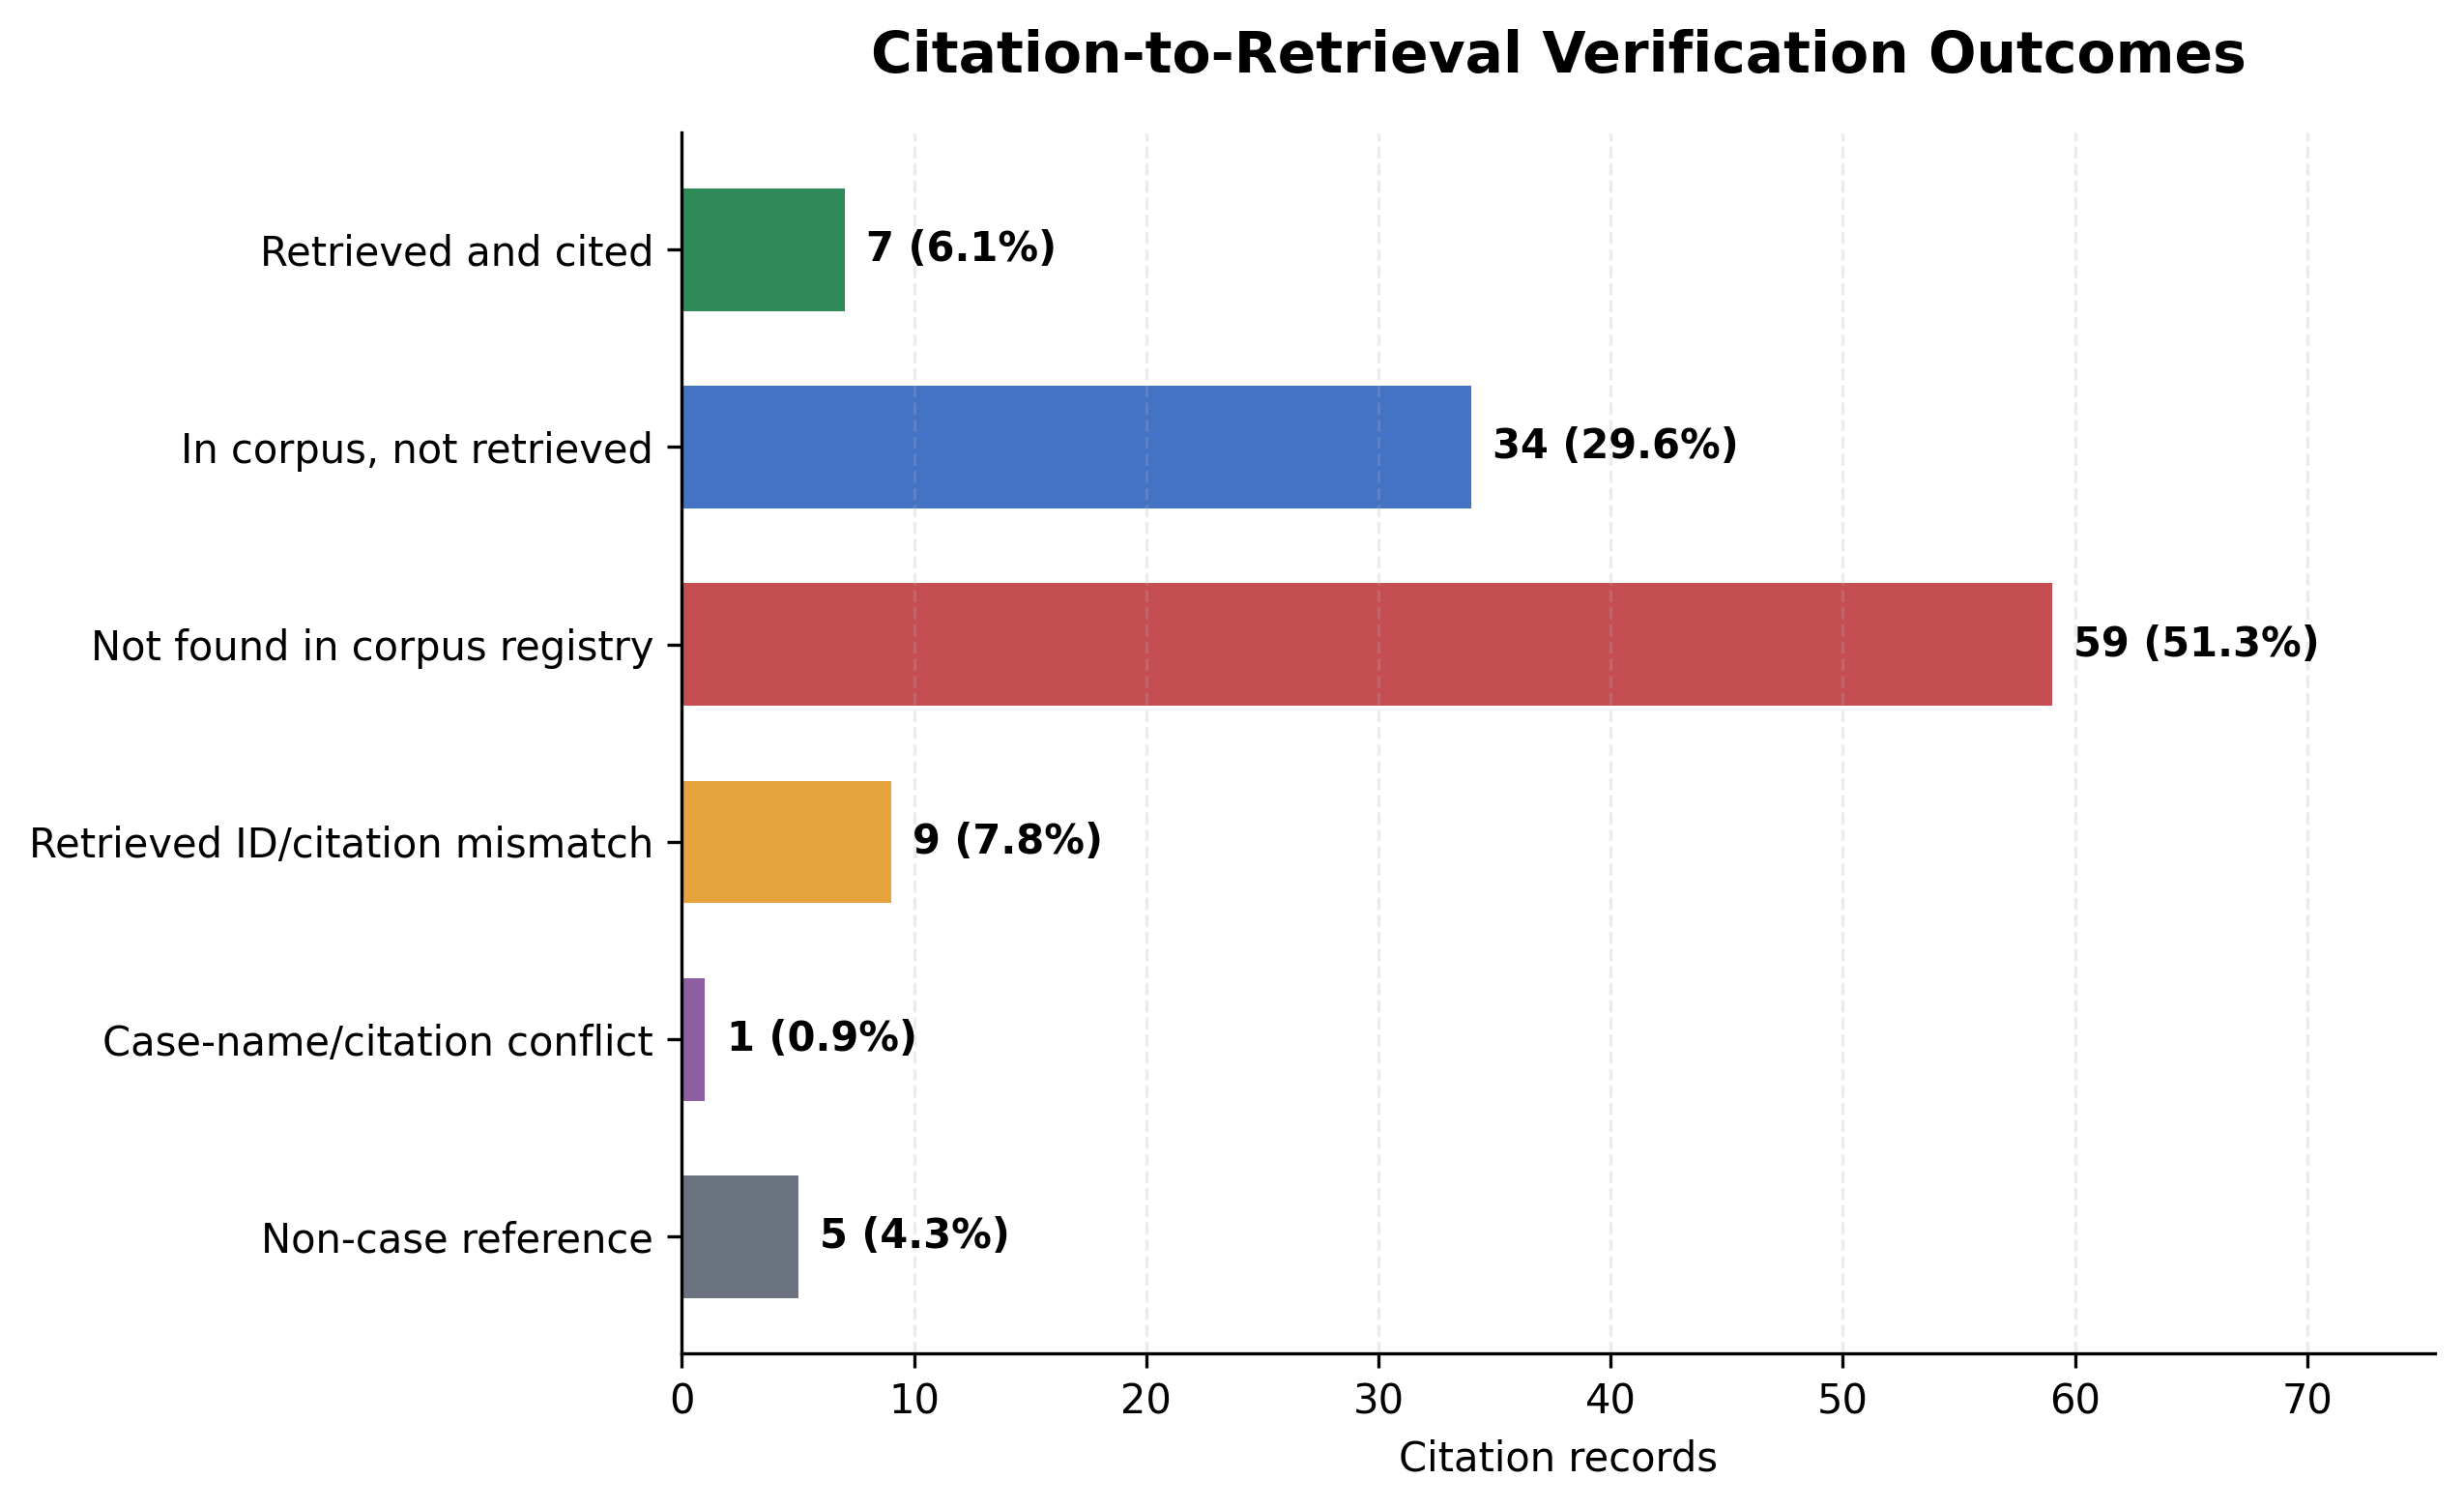
\includegraphics[width=0.70\textwidth]{figure_3_retrieval_outcomes.png}
\caption{Citation-to-retrieval verification outcomes ($n = 115$). Case-law analysis in the text uses $n = 110$, excluding five non-case references.}
\label{fig:retrieval-outcomes}
\end{figure*}

The case-law subset contained 61 occurrences from real-case inputs and 49 from synthetic-case inputs. Twenty-eight of the 61 real-case citations (45.9\%) were not found in the frozen Neon registry, compared with 31 of the 49 synthetic-case citations (63.3\%). The observed difference was 17.4 percentage points. Because the dataset contains repeated runs and was not designed as an independent comparison between input types, this difference is reported descriptively and is not treated as evidence of a causal effect.

\subsection{Layer 2: External Citation and Holding Accuracy}

The 115 citation occurrences were consolidated into 35 distinct authority or reference groups. Of these, 33 were case-law authorities and 2 were non-case references. Every distinct case-law authority was checked manually against BAILII and supplementary legal sources~\cite{bailii}. Thirty-two of the 33 case-law authorities were located externally, while one remained ambiguous. No case in the sample was confirmed as fabricated.

A separate citation-form assessment across all 35 groups found 23 (65.7\%) correct and complete, 8 (22.9\%) incomplete, and 4 (11.4\%) incorrect. These results concern citation form rather than holding accuracy.

Holding accuracy was evaluated for the 98 citation occurrences in the validation sample. Across all 98 occurrences, 47 (48.0\%) received a final label of accurate, 30 (30.6\%) were partially accurate, 17 (17.3\%) were inaccurate, and 4 (4.1\%) were not applicable. Figure~\ref{fig:human-labels}(a) presents this complete distribution.

After excluding the four non-applicable occurrences, 94 holding attributions remained assessable. Among these, 47 (50.0\%) were accurate, 30 (31.9\%) were partially accurate, and 17 (18.1\%) were inaccurate. The combined holding-defect rate was therefore 47 of 94 assessable occurrences (50.0\%; 95\% CI: 40.1\%--59.9\%).

The errors ranged from imprecise descriptions of a relevant principle to the use of authorities from unrelated areas of law. In the most serious example, the generated proposition reversed the effect of the cited decision. Table~\ref{tab:misattributions} provides four representative examples.

\begin{table*}[t]
\centering
\small
\caption{Representative manually verified holding misattributions}
\label{tab:misattributions}
\begin{tabular}{p{3.4cm}p{3.9cm}p{5.2cm}p{2.3cm}}
\toprule
\textbf{Authority} & \textbf{Principle attributed by Hercules} & \textbf{Subject and holding of the authority} & \textbf{Classification} \\
\midrule
\textit{Gorringe v Calderdale Metropolitan Borough Council} [2004] UKHL 15~\cite{gorringe2004}
& A highway authority has a duty to ensure road safety.
& The House of Lords held that the council did not owe the claimant a duty to place a road marking or warning sign at the accident location.
& Holding reversed \\
\addlinespace
\textit{Chapman v Mid \& South Essex NHS Foundation Trust} [2023] EWHC 1290 (KB)~\cite{chapman2023}
& Statutory control over public safety for cyclists and pedestrians.
& A clinical-negligence case concerning delayed diagnosis and treatment of a spinal condition, unrelated to highway safety.
& Wrong area of law \\
\addlinespace
\textit{Bank St Petersburg PJSC v Arkhangelsky} [2020] EWCA Civ 408~\cite{bankstpetersburg2020}
& Statutory defences must be examined for reasonableness and due diligence.
& A commercial dispute addressing the evaluation and standard of proof where dishonesty was alleged.
& Wrong area of law \\
\addlinespace
\textit{Chartbrook Ltd v Persimmon Homes Ltd} [2009] UKHL 38~\cite{chartbrook2009}
& Courts may imply reasonable pricing terms where the contract is unclear.
& A decision concerning contractual interpretation and the correction of drafting language, rather than the implication of reasonable pricing terms.
& Wrong principle \\
\bottomrule
\end{tabular}
\end{table*}

The provenance data help distinguish different sources of error. \textit{Gorringe} and \textit{Chartbrook} were both classified as retrieved and cited, yet their holding attributions were inaccurate. Their misdescription cannot therefore be explained solely by retrieval absence. By contrast, \textit{Chapman} was not found in the frozen Neon registry and was not present in the linked retrieval. This occurrence combines a registry-provenance gap with an inaccurate attribution.

\subsection{Layer 3: Reasoning Grounding}

Reasoning grounding was evaluated across all 98 validation occurrences. Eighty-four occurrences (85.7\%; 95\% CI: 77.4\%--91.3\%) were labelled ungrounded, 11 (11.2\%) were partially grounded, and only 3 (3.1\%) were fully grounded in the retrieved passages. Figure~\ref{fig:human-labels}(b) presents this distribution.

Among the 55 real-case validation occurrences, 45 (81.8\%) were ungrounded, compared with 39 of 43 (90.7\%) for synthetic inputs. As with the Layer~1 comparison, the difference is reported descriptively because the dataset was not designed as an independent comparison between input types.

\begin{figure*}[t]
\centering
\begin{minipage}[t]{0.49\textwidth}
\centering
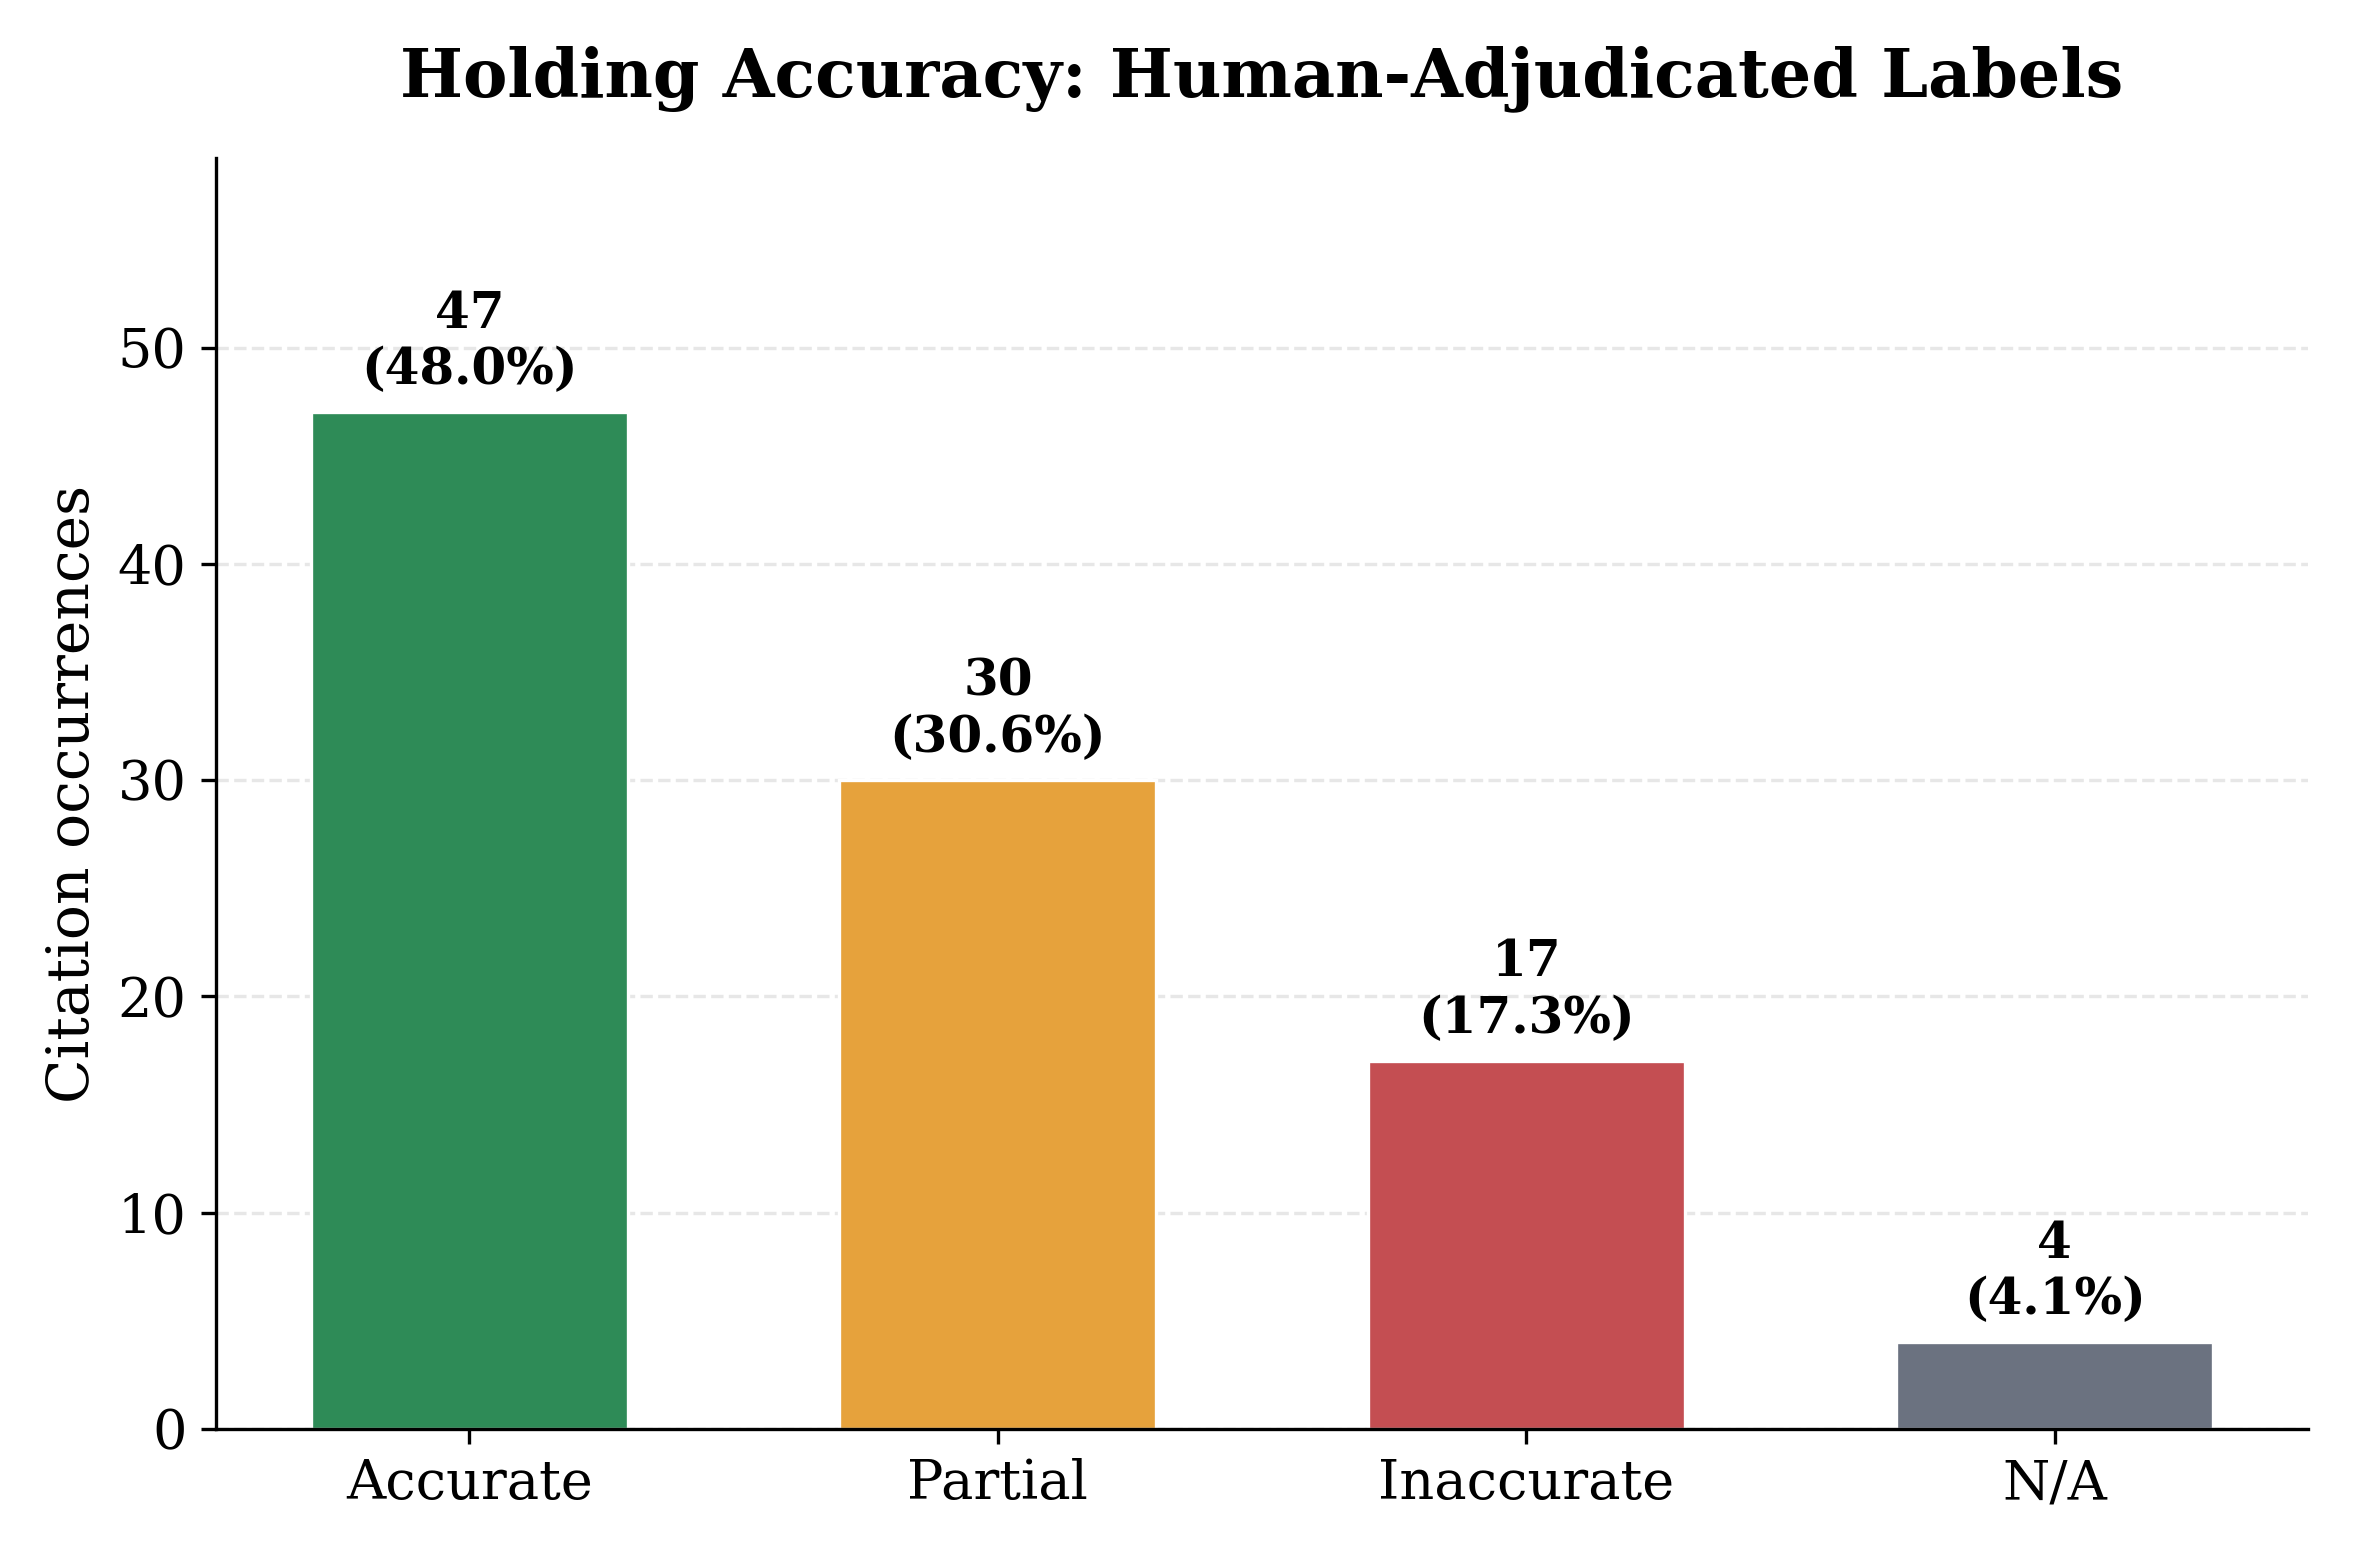
\includegraphics[width=\linewidth]{figure_4_holding_accuracy.png}

\small (a) Holding-accuracy labels for all 98 validation occurrences
\end{minipage}
\hfill
\begin{minipage}[t]{0.49\textwidth}
\centering
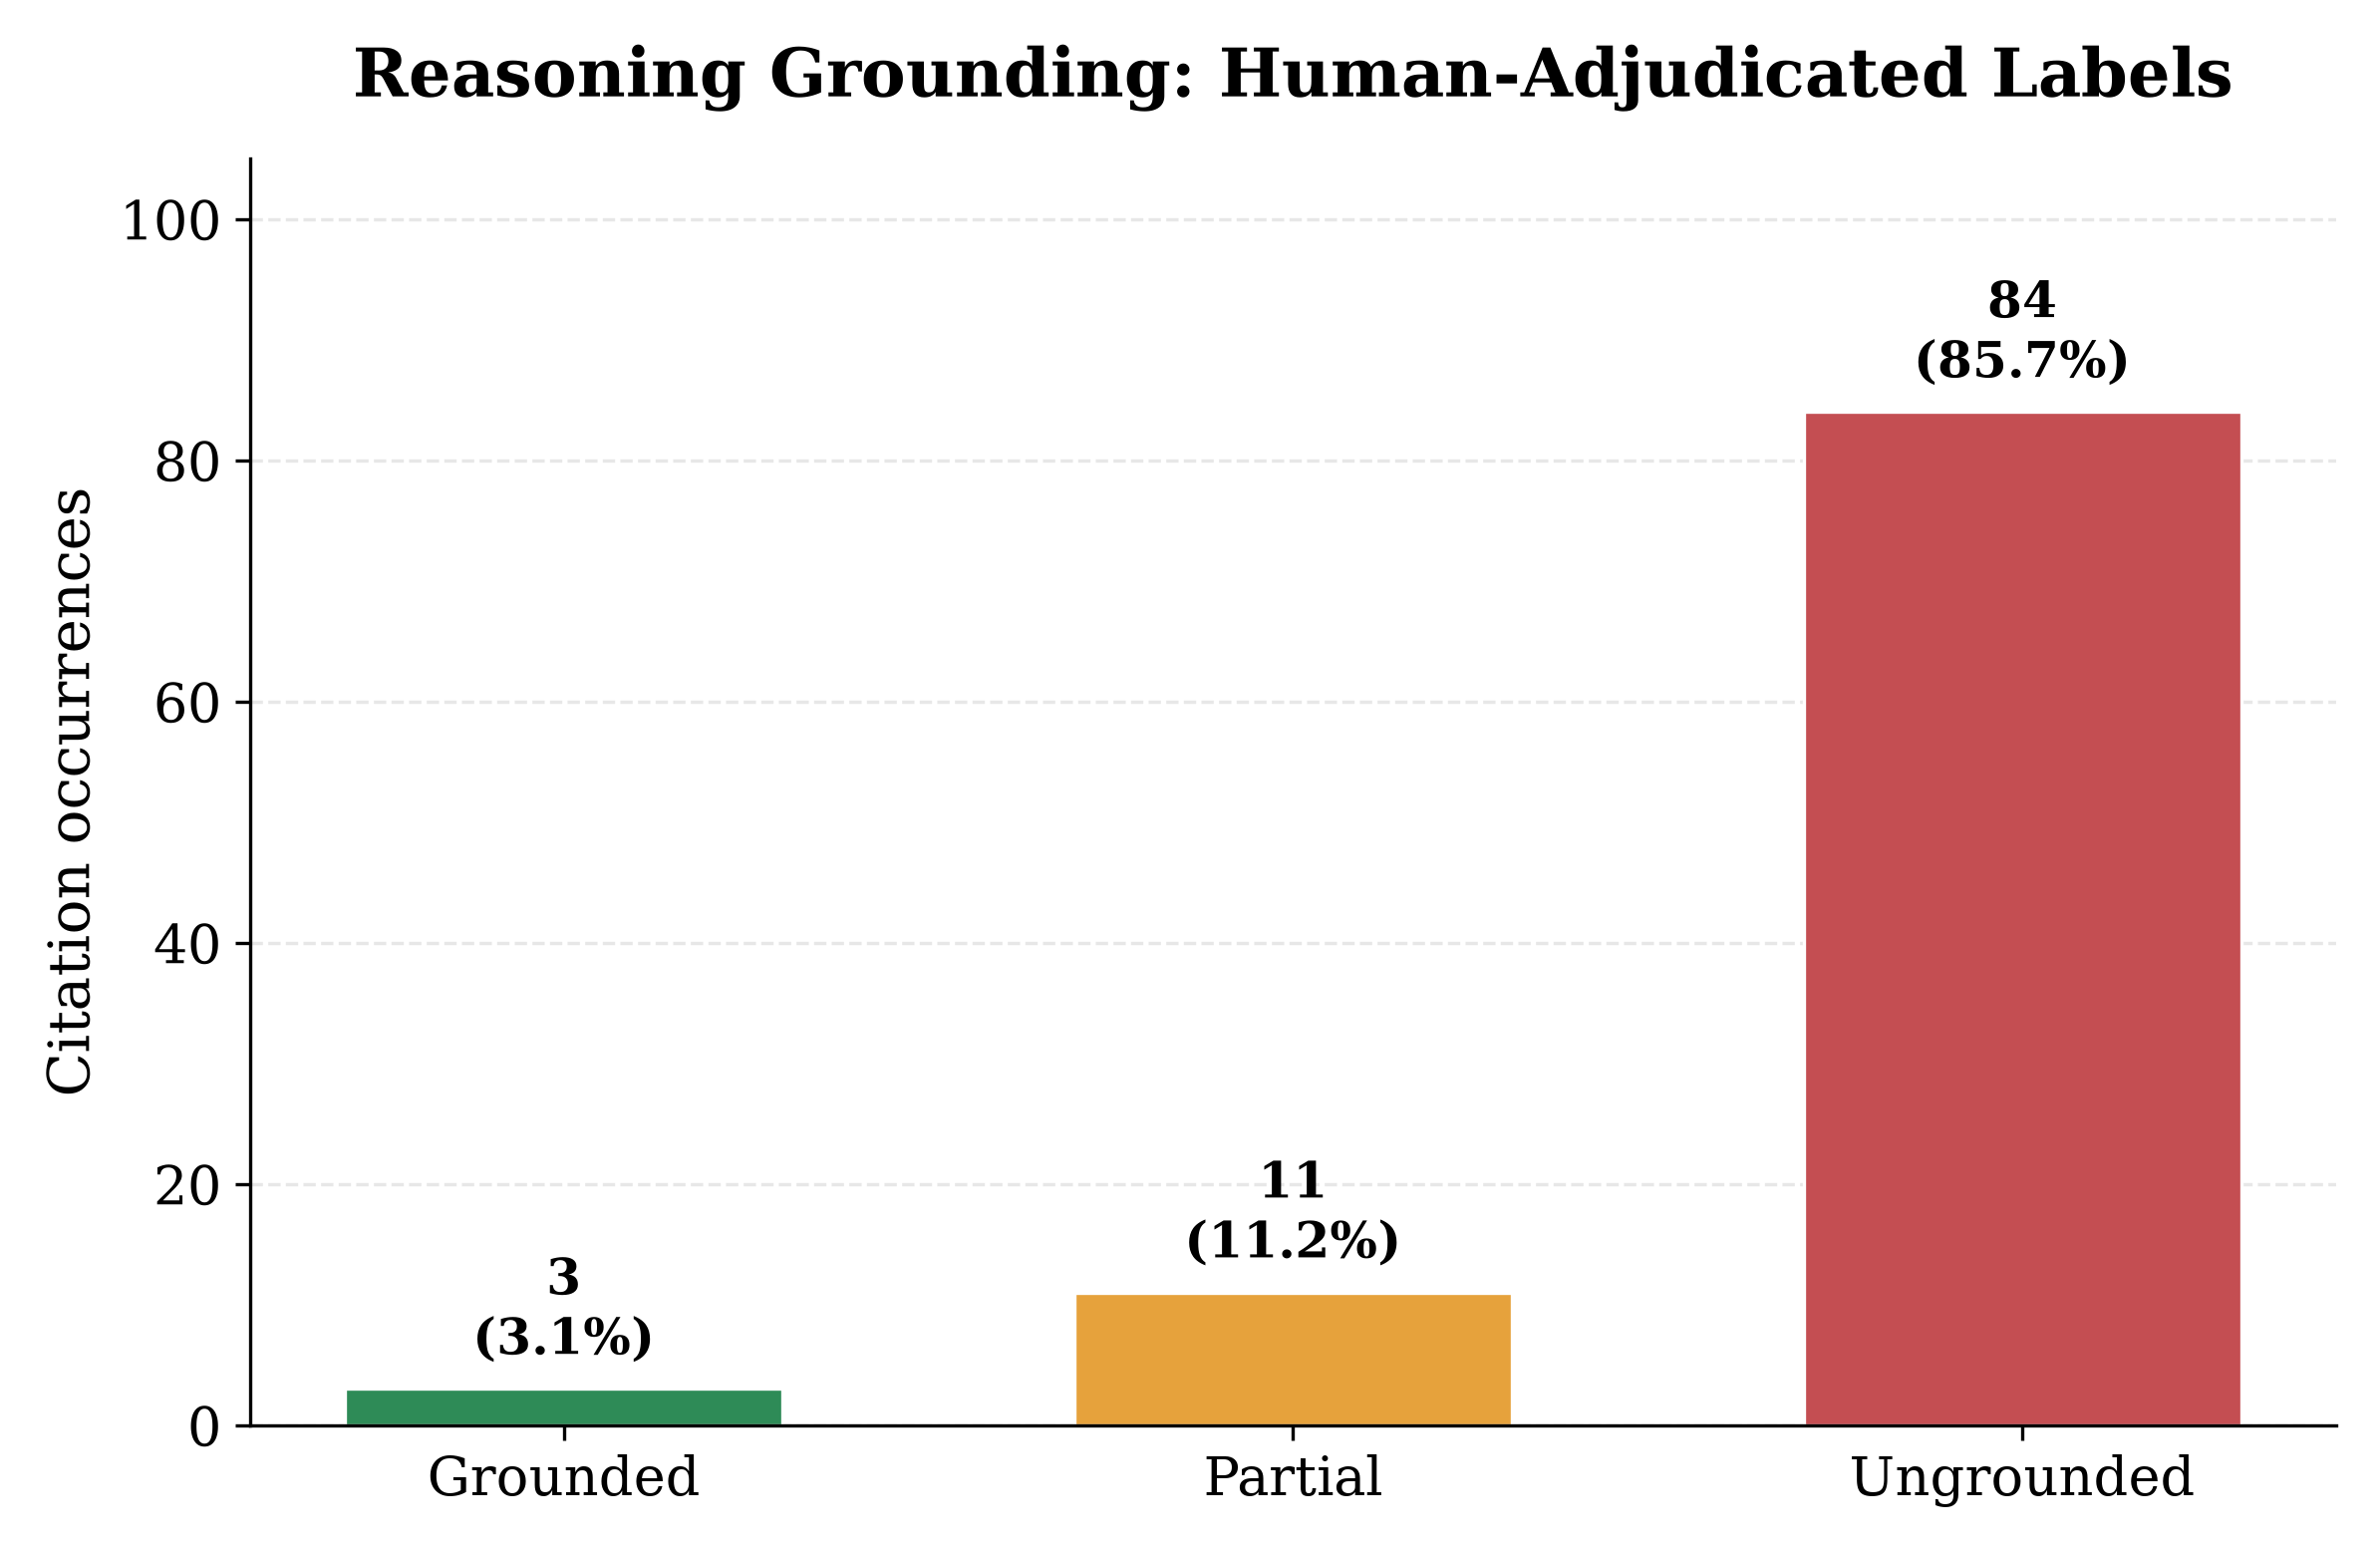
\includegraphics[width=\linewidth]{figure_5_reasoning_grounding.png}

\small (b) Reasoning-grounding labels for all 98 validation occurrences
\end{minipage}
\caption{Final author-adjudicated reference labels. Holding accuracy includes four non-applicable occurrences, while reasoning grounding was applicable to all 98 occurrences.}
\label{fig:human-labels}
\end{figure*}

\subsection{Agreement Between Annotation Passes}

Agreement between the primary human R1 annotation and the AI-assisted R2 pass was calculated descriptively using Cohen's Kappa~\cite{cohen1960}. For holding accuracy, 79 of 94 assessable label pairs agreed, giving observed agreement of 84.0\% and $\kappa = 0.74$. For reasoning grounding, 40 of 98 pairs agreed, giving observed agreement of 40.8\% and $\kappa = 0.054$. Under the commonly used Landis and Koch descriptors, these values correspond to substantial and slight agreement, respectively~\cite{landis1977}. They do not represent inter-human reliability.

The grounding disagreements were concentrated at the boundary between partial and ungrounded. Of the 58 grounding disagreements, 54 involved R1 assigning \textit{partial} and R2 assigning \textit{no}. Final failure-rate estimates use the author-adjudicated labels, but the low initial grounding agreement means that the 85.7\% ungrounded estimate should be interpreted as an adjudicated result rather than an uncontested classification.

\subsection{Verifier Validation}

The primary verifier evaluation used the frozen V1 predictions. Predictions were compared with the final adjudicated reference labels for the 98 validation occurrences. Table~\ref{tab:validation} summarises the results.

\begin{table}[t]
\centering
\caption{Automated verifier performance on the validation sample}
\label{tab:validation}
\begin{tabular}{lccc}
\toprule
\textbf{Dimension} & \textbf{Accuracy} & \textbf{$\kappa$} & \textbf{Interpretation} \\
\midrule
Citation status & 87.8\% & 0.80 & Substantial \\
Holding accuracy & 4.1\% & 0.04 & Slight \\
Reasoning grounding & 85.7\% & 0.24 & Fair \\
\bottomrule
\end{tabular}
\end{table}

The citation-status verifier correctly classified 86 of 98 occurrences, producing exact accuracy of 87.8\%, $\kappa = 0.80$, and macro $F_1 = 0.71$ across the five validation classes (the mismatch class contributed $F_1 = 0$). It performed strongly for the two largest classes: \textit{not found in the frozen Neon registry} ($F_1 = 0.90$) and \textit{in the structured registry, not retrieved} ($F_1 = 0.98$).

Performance was weaker for less frequent failure types. The validation sample contained seven retrieved-ID and citation-mismatch occurrences, but the verifier identified none of them correctly. The aggregate result was driven mainly by the two largest citation-status classes. Citation-status automation was therefore useful for initial registry and retrieval screening, but it was not reliable for every mismatch category.

For holding accuracy, the verifier returned \textit{unclear} for all 94 substantive occurrences because authoritative judgment text was unavailable. It correctly classified only the four non-applicable references, resulting in accuracy of 4.1\% and $\kappa = 0.04$. The result represents complete abstention on assessable holding claims rather than successful automated holding verification.

For reasoning grounding, the verifier correctly classified 84 of 98 occurrences, giving accuracy of 85.7\% and $\kappa = 0.24$. It predicted \textit{no} for 92 occurrences, \textit{partial} for 6, and \textit{yes} for none. It correctly identified 3 of the 11 partially grounded occurrences and none of the 3 fully grounded occurrences.

Because 84 of the 98 adjudicated grounding labels were \textit{no}, an always-\textit{no} baseline would also have achieved 85.7\% accuracy. The verifier's headline accuracy therefore does not demonstrate useful discrimination across the grounding classes.

In a post hoc V3 sensitivity check, supplying the exported Qdrant authority text increased holding exact accuracy from 4.1\% to 10.2\%, while Kappa decreased from 0.04 to approximately 0.002. This did not constitute a meaningful improvement and did not alter the decision to retain V1 as the primary result.

\subsection{Recurring Default Authorities}

Two authorities concerning the judicial duty to give reasons recurred frequently: \textit{English v Emery Reimbold \& Strick Ltd} appeared in 22 judgments and \textit{Flannery v Halifax Estate Agencies Ltd} in 25~\cite{english2002,flannery1999}. At least one appeared in 30 of 59 judgments (50.8\%). Their use was not consistently accurate: among 21 labelled \textit{Flannery} occurrences, 9 were accurate, 8 partially accurate, and 4 inaccurate. The frequency suggests a possible default citation pattern, but relevance to the underlying dispute was not annotated as a separate variable.

\section{Discussion}

\subsection{The Risk Lies Beyond Fabrication}

One of the clearest findings is what was not observed. Of the 33 distinct case-law authorities examined, 32 were located in external legal sources and one remained ambiguous. No citation was confirmed as fabricated. This should not be interpreted as evidence that the system could never invent a case. It means only that no fabricated case was identified in this sample.

An audit based solely on whether a cited case exists would therefore have presented an incomplete picture. Previous research has similarly found that retrieval-augmented legal systems can produce unsupported answers even when their citations appear credible~\cite{magesh2024}. In this study, the principal problem was not the existence of the authorities, but the accuracy of the propositions attributed to them.

Among the 94 assessable holding attributions, 47 were accurate, 30 were partially accurate, and 17 were inaccurate. The combined holding-defect rate was therefore 50.0\%. A genuine citation did not guarantee that the authority had been represented faithfully. This distinction matters because a real case gives an inaccurate proposition an appearance of legitimacy that an obviously fabricated citation would not possess.

At judgment level, 29 of 50 validation judgments (58.0\%) contained at least one holding defect, and 48 of 50 (96.0\%) contained at least one ungrounded reasoning step. From an operational perspective, nearly every validation draft judgment exhibited at least one unsupported legal proposition.

\subsection{What the Individual Cases Show}

The individual cases illustrate how this problem appeared in practice. \textit{Gorringe v Calderdale Metropolitan Borough Council} was cited twice, and both holding attributions were labelled inaccurate. The House of Lords held that the council did not owe the claimant a duty to place a road marking or warning sign at the location of the accident~\cite{gorringe2004}. The generated judgments used the case to support a positive duty concerning road safety, which reversed the effect of the decision.

In one of the same drafts, \textit{Yetkin v London Borough of Newham} was labelled only partially accurate~\cite{yetkin2010}. This shows that the system's treatment of authorities was not consistently correct or consistently incorrect, even within a short group of citations. That variation makes the errors more difficult to identify through superficial review.

Other cases showed a similar pattern. The neutral citation attributed to \textit{Chapman v Mid \& South Essex NHS Foundation Trust} [2023] EWHC 1290 (KB) concerns a clinical-negligence dispute involving delayed diagnosis and treatment~\cite{chapman2023}. It was nevertheless used to support a proposition concerning highway safety. \textit{Chartbrook Ltd v Persimmon Homes Ltd}, a decision concerning contractual interpretation, was also assigned an inaccurate holding and ungrounded reasoning in the annotation data~\cite{chartbrook2009}. These examples show that the system could identify a real authority while failing to preserve its legal meaning.

\subsection{A Grounding Problem, Not Only a Retrieval Problem}

The results also separate retrieval failure from evidence-use failure. At Layer 1, 59 of 110 case-law citation occurrences (53.6\%) were not found in the frozen Neon registry and were not present in the linked retrieval. Because the Neon and Qdrant stores had different coverage, this finding is a provenance gap rather than proof that all 59 authorities were absent from the complete Qdrant knowledge base.

Registry and retrieval coverage do not explain the complete result. Some inaccurately described authorities, including \textit{Gorringe} and \textit{Chartbrook}, were linked to retrieved material. In addition, 84 of 98 annotated reasoning occurrences (85.7\%) were classified as ungrounded, while only 3 were fully grounded and 11 were partially grounded. The problem therefore concerned both access to linked evidence and the system's use of that evidence.

This distinction reflects the broader separation between retrieval quality and generation faithfulness in RAG evaluation~\cite{ragas2024}. Better retrieval may reduce the number of citations lacking clear provenance, but it cannot ensure that the generator describes a retrieved authority correctly. The results do not establish that every error originated solely in the language model, since the corpus also contained processed chunks and generated metadata rather than complete authoritative judgments in every instance. They do show that improving retrieval alone would not resolve the observed failures.

\subsection{What the Verifier Can and Cannot Do}

The verifier performed well at broad citation-status classification. It correctly classified 86 of the 98 validation occurrences, giving an accuracy of 87.8\% and Cohen's Kappa of $\kappa = 0.80$. This result supports the automation of checks such as whether an authority can be matched to the structured registry and whether it was retrieved.

The aggregate score nevertheless hides an important weakness. The validation sample contained seven retrieved-ID and citation-mismatch occurrences, and the verifier correctly identified none of them. Its strong overall result was driven mainly by the two largest classes: authorities not matched to the frozen Neon registry and authorities present in the registry but not retrieved. Citation-status checking can therefore be automated as an initial screening step, but the current verifier should not be treated as reliable for every failure category.

The limits were clearer for the other two layers. For holding accuracy, the verifier returned \textit{unclear} for all 94 substantive occurrences because authoritative judgment text was unavailable. Its 4.1\% accuracy resulted only from correctly identifying the four non-applicable rows. This abstention was preferable to inventing an answer, but it meant that the verifier did not automate substantive holding assessment.

For reasoning grounding, the verifier obtained 85.7\% accuracy but only fair agreement with the adjudicated labels ($\kappa = 0.24$). The accuracy equalled the result that would have been obtained by predicting the majority \textit{no} class for every occurrence. The verifier identified none of the three fully grounded occurrences and only three of the eleven partially grounded occurrences. The headline accuracy should therefore not be interpreted as strong grounding performance.

Holding labels were more consistent across the two annotation passes than grounding labels. R1 and the AI-assisted R2 pass agreed on 84.0\% of assessable holding labels, with $\kappa = 0.74$. For reasoning grounding, agreement was 40.8\% and $\kappa = 0.054$. The final grounding labels were selected through author adjudication, but the low initial agreement shows that grounding is difficult and judgment-dependent. Manual review remains necessary, but it should be supported by a clear codebook, access to the same evidence, and documented adjudication. Similar reliance on human evaluation has been reported in previous work on factuality and legal-AI reliability~\cite{maynez2020,magesh2024}.

\subsection{Implications for Deployment}

The findings support several practical safeguards. A generated judgment should identify the exact passage used to support each legal proposition rather than provide only a case name or citation. The system should abstain when authoritative text is unavailable, and citations should not be presented as grounded unless the corresponding authority was actually retrieved. Corpus versions, retrieval results, and source identifiers should also be retained so that each proposition can be audited later.

Human oversight should focus on the meaning and relevance of the cited authority, not simply whether the citation exists. This is particularly important in judicial decision support, where a genuine but misrepresented authority may influence the legal analysis while remaining difficult to detect.

The conversion of skeleton arguments from unstructured PDF files into structured XML creates an additional operational risk. Paragraphs, citations, and case metadata must be preserved during conversion and checked before generation. Judicial names and panel information should likewise be drawn from validated metadata rather than generated freely. These controls would not eliminate every error, but they would make unsupported claims easier to identify before a draft judgment reached a judicial user.

\section{Conclusion}

This study examined the accuracy and reliability of 59 AI-generated draft judgments produced by Hercules. The audit covered 115 citation occurrences across three layers: whether cited cases could be linked to the frozen structured registry and retrieval records, whether the cases were described accurately, and whether the reasoning was supported by the retrieved passages. All 33 distinct case-law authorities were checked manually against external legal sources, and 98 citation occurrences were annotated for holding accuracy and reasoning grounding.

Taken together, the findings point to a clear reliability problem. No case was confirmed as fabricated. Of the 33 distinct case-law authorities, 32 were located externally and one remained ambiguous. However, the absence of fabricated cases did not make the judgments reliable. Fifty-nine of 110 case-law citations (53.6\%) could not be matched to the frozen Neon registry and were not present in the linked retrieval. Of the 94 assessable holding attributions, 47 (50.0\%) were inaccurate or only partially accurate. In addition, 84 of 98 reasoning occurrences (85.7\%) were not grounded in the retrieved passages.

This is a particularly concerning type of failure because real citations can be more dangerous than fabricated ones. A fabricated case name is detectable through a simple existence check; a genuine authority cited for a proposition it does not establish carries apparent legitimacy that resists superficial review. The language is confident, the reasoning resembles conventional legal writing, and a reader may accept the proposition without noticing the misattribution.

The automated verifier performed well when screening citation status against the frozen registry and retrieval records, achieving 87.8\% accuracy and substantial agreement with the adjudicated reference statuses ($\kappa = 0.80$). It was much less successful at assessing holding accuracy ($\kappa = 0.04$) and reasoning grounding ($\kappa = 0.24$). These results suggest that automated checks can support citation and retrieval-provenance screening, but manual legal judgment remains necessary when evaluating the meaning of an authority and the reasoning based upon it.

The study is limited by its modest, partly non-independent dataset, a single generation model, and coverage differences between the Qdrant knowledge base and frozen Neon registry. Future work should use a larger sample of real cases, supply authoritative full-text judgments for automated holding checks, and compare retrieval depths, prompts, and models. The central lesson is that the most important observed risk was not an invented case, but a real case cited for a proposition it does not establish.

\section*{Acknowledgment}

The author gratefully acknowledges Professor Jun Liu, School of Computing, Ulster University, for his supervision, constructive feedback, and guidance. The author also thanks John Keers BL and John McCord at the Centre for Legal Technology, Ulster University, for providing access to the Hercules research prototype and for their review and feedback on this work. Appreciation is extended to those who supported the verification of legal authorities. Finally, the author acknowledges the developers of the Cambridge Law Corpus~\cite{cambridge2023}, which provided an important data resource.

\section*{AI Tools Statement}

Generative AI was used during manuscript preparation for language editing, restructuring, code assistance, and an AI-assisted second annotation pass. The author checked the cited legal sources, reviewed the annotation evidence, selected the final adjudicated reference labels, verified the reported calculations, and takes responsibility for the analysis and conclusions.

\vspace{-4pt}
\begin{thebibliography}{99}

\bibitem{hercules}
Centre for Legal Technology, Ulster University, ``AI in Judicial Decision-Making: Hercules AI Decision-Making Assistant.'' [Online]. Available: \url{https://www.ulster.ac.uk/research/topic/law/centre-for-legal-technology/projects/ai-in-judicial-decision-making}

\bibitem{magesh2024}
V. Magesh, F. Surani, M. Dahl, M. Suzgun, C. D. Manning, and D. E. Ho, ``Hallucination-free? Assessing the reliability of leading AI legal research tools,'' arXiv:2405.20362, 2024.

\bibitem{maynez2020}
J. Maynez, S. Narayan, B. Bohnet, and R. McDonald, ``On faithfulness and factuality in abstractive summarization,'' in \textit{Proc. 58th Annual Meeting of the Association for Computational Linguistics}, 2020, pp. 1906--1919.

\bibitem{huang2023}
L. Huang \textit{et al.}, ``A survey on hallucination in large language models: Principles, taxonomy, challenges, and open questions,'' arXiv:2311.05232, 2023.

\bibitem{ji2023}
Z. Ji \textit{et al.}, ``Survey of hallucination in natural language generation,'' \textit{ACM Computing Surveys}, vol. 55, no. 12, art. 248, pp. 1--38, 2023.

\bibitem{zhang2023}
Y. Zhang \textit{et al.}, ``Siren's song in the AI ocean: A survey on hallucination in large language models,'' arXiv:2309.01219, 2023.

\bibitem{dahl2024}
M. Dahl, V. Magesh, M. Suzgun, and D. E. Ho, ``Large legal fictions: Profiling legal hallucinations in large language models,'' \textit{Journal of Legal Analysis}, vol. 16, no. 1, pp. 64--93, 2024.

\bibitem{nigam2024}
S. K. Nigam, A. Deroy, S. Maity, and A. Bhattacharya, ``Rethinking legal judgement prediction in a realistic scenario in the era of large language models,'' in \textit{Proc. Natural Legal Language Processing Workshop 2024}, 2024, pp. 61--80, doi: 10.18653/v1/2024.nllp-1.6.

\bibitem{ukjudicial2025}
UK Judicial Office, ``Artificial intelligence: Judicial guidance,'' Oct. 2025. [Online]. Available: \url{https://www.judiciary.uk/guidance-and-resources/artificial-intelligence-ai-judicial-guidance-october-2025/}

\bibitem{gao2024}
Y. Gao \textit{et al.}, ``Retrieval-augmented generation for large language models: A survey,'' arXiv:2312.10997, 2024.

\bibitem{ragas2024}
S. Es, J. James, L. Espinosa-Anke, and S. Schockaert, ``RAGAS: Automated evaluation of retrieval augmented generation,'' in \textit{Proc. 18th Conf. European Chapter of the Association for Computational Linguistics: System Demonstrations}, 2024, pp. 150--158, doi: 10.18653/v1/2024.eacl-demo.16.

\bibitem{rashkin2023}
H. Rashkin, V. Nikolaev, M. Lamm, L. Aroyo, M. Collins, D. Das, S. Petrov, G. S. Tomar, I. Turc, and D. Reitter, ``Measuring attribution in natural language generation models,'' \textit{Computational Linguistics}, vol. 49, no. 4, pp. 777--806, 2023.

\bibitem{cambridge2023}
A. \"{O}stling, H. Sargeant, H. Xie, L. Bull, A. Terenin, L. Jonsson, M. Magnusson, and F. Steffek, ``The Cambridge Law Corpus: A dataset for legal AI research,'' in \textit{Advances in Neural Information Processing Systems 36}, 2023, pp. 41355--41385.

\bibitem{bailii}
British and Irish Legal Information Institute, ``British and Irish Legal Information Institute.'' [Online]. Available: \url{https://www.bailii.org/}

\bibitem{codebook}
R. Raj, ``Hercules holding-accuracy and reasoning-grounding codebook,'' version 1.1, project supplementary material, 2026.

\bibitem{cohen1960}
J. Cohen, ``A coefficient of agreement for nominal scales,'' \textit{Educational and Psychological Measurement}, vol. 20, no. 1, pp. 37--46, 1960.

\bibitem{landis1977}
J. R. Landis and G. G. Koch, ``The measurement of observer agreement for categorical data,'' \textit{Biometrics}, vol. 33, no. 1, pp. 159--174, 1977.

\bibitem{gorringe2004}
\textit{Gorringe v Calderdale Metropolitan Borough Council}, [2004] UKHL 15, House of Lords, Apr. 1, 2004. [Online]. Available: \url{https://www.bailii.org/uk/cases/UKHL/2004/15.html}

\bibitem{chapman2023}
\textit{Chapman v Mid \& South Essex NHS Foundation Trust}, [2023] EWHC 1290 (KB), High Court of Justice, May 30, 2023. [Online]. Available: \url{https://www.bailii.org/ew/cases/EWHC/KB/2023/1290.html}

\bibitem{bankstpetersburg2020}
\textit{Bank St Petersburg PJSC v Arkhangelsky}, [2020] EWCA Civ 408, Court of Appeal, Mar. 18, 2020. [Online]. Available: \url{https://www.bailii.org/ew/cases/EWCA/Civ/2020/408.html}

\bibitem{chartbrook2009}
\textit{Chartbrook Ltd v Persimmon Homes Ltd}, [2009] UKHL 38, House of Lords, July 1, 2009. [Online]. Available: \url{https://www.bailii.org/uk/cases/UKHL/2009/38.html}

\bibitem{english2002}
\textit{English v Emery Reimbold \& Strick Ltd}, [2002] EWCA Civ 605, Court of Appeal, Apr. 30, 2002. [Online]. Available: \url{https://www.bailii.org/ew/cases/EWCA/Civ/2002/605.html}

\bibitem{flannery1999}
\textit{Flannery v Halifax Estate Agencies Ltd}, [1999] EWCA Civ 811; [2000] 1 WLR 377, Court of Appeal, Feb. 18, 1999. [Online]. Available: \url{https://www.bailii.org/ew/cases/EWCA/Civ/1999/811.html}

\bibitem{yetkin2010}
\textit{Yetkin v London Borough of Newham}, [2010] EWCA Civ 776, Court of Appeal, July 6, 2010. [Online]. Available: \url{https://www.bailii.org/ew/cases/EWCA/Civ/2010/776.html}

\end{thebibliography}

\end{document}